\documentclass[12pt,a4paper]{article}
\usepackage{amsmath,amscd,amsbsy,amssymb,latexsym,url,bm,amsthm}
\usepackage{epsfig,graphicx,subfigure}
\usepackage{enumitem,balance}
\usepackage{wrapfig}
\usepackage{mathrsfs,euscript}
\usepackage[usenames]{xcolor}
\usepackage{hyperref}
\usepackage[vlined,ruled,linesnumbered]{algorithm2e}
\usepackage{array}
\hypersetup{colorlinks=true,linkcolor=black}

\newtheorem{theorem}{Theorem}
\newtheorem{lemma}[theorem]{Lemma}
\newtheorem{proposition}[theorem]{Proposition}
\newtheorem{corollary}[theorem]{Corollary}
\newtheorem{exercise}{Exercise}
\newtheorem*{solution}{Solution}
\newtheorem{definition}{Definition}
\theoremstyle{definition}

\renewcommand{\thefootnote}{\fnsymbol{footnote}}

\newcommand{\postscript}[2]
 {\setlength{\epsfxsize}{#2\hsize}
  \centerline{\epsfbox{#1}}}

\renewcommand{\baselinestretch}{1.0}

\setlength{\oddsidemargin}{-0.365in}
\setlength{\evensidemargin}{-0.365in}
\setlength{\topmargin}{-0.3in}
\setlength{\headheight}{0in}
\setlength{\headsep}{0in}
\setlength{\textheight}{10.1in}
\setlength{\textwidth}{7in}
\makeatletter \renewenvironment{proof}[1][Proof] {\par\pushQED{\qed}\normalfont\topsep6\p@\@plus6\p@\relax\trivlist\item[\hskip\labelsep\bfseries#1\@addpunct{.}]\ignorespaces}{\popQED\endtrivlist\@endpefalse} \makeatother
\makeatletter
\renewenvironment{solution}[1][Solution] {\par\pushQED{\qed}\normalfont\topsep6\p@\@plus6\p@\relax\trivlist\item[\hskip\labelsep\bfseries#1\@addpunct{.}]\ignorespaces}{\popQED\endtrivlist\@endpefalse} \makeatother

\begin{document}
\noindent

%========================================================================
\noindent\framebox[\linewidth]{\shortstack[c]{
\Large{\textbf{Lab09-Approximation Algorithm}}\vspace{1mm}\\
CS214-Algorithm and Complexity, Xiaofeng Gao, Spring 2019.}}
\begin{center}
\footnotesize{\color{red}$*$ If there is any problem, please contact TA Jiahao Fan.}

% Please write down your name, student id and email.
\footnotesize{\color{blue}$*$ Name: KylinChen  \quad Student ID: 517030910155 \quad Email: 
k1017856853@icloud.com}
\end{center}

\begin{enumerate}
    \item
    \textbf{Metric $k$-center:} Let $G = (V, E)$ be an complete undirected graph with nonnegative edge costs satisfying the triangle inequality, and $k$ be a positive integer. For any set $S \subseteq V$ and vertex $v \in V$, define $cost(v,S)$ to be the cost of the cheapest edge from $v$ to a vertex in $S$ ($cost(v, S) = 0$ if $v \in S$). The problem is to find a set $S \subseteq V$, with $|S| = k$, so as to minimize $\max_v\{cost(v, S)\}$.

    \begin{enumerate}
        \item
        Design a greedy approximation algorithm (in the form of pseudo code) with approximation ratio $2$ for this problem.

        (Basic idea: start with an arbitrary center, and in each round, add the `farthest' vertex to the center set until there are totaly $k$ centers)

        \item
        Prove that your greedy algorithm achieves an approximation ratio of 2 for the metric $k$-center problem. (Hint: prove by contradiction and use the triangle inequality.)
    \end{enumerate}

    \begin{solution}\item
    \renewcommand{\qedsymbol}{}
    \begin{itemize}
    \item [(a)] We can get a feasible solution by simple steps below:\par
    \begin{itemize}
    \item Choose the first center arbitrarily.
    \item At every step, choose the vertex that is furthest from the current centers to become a center.
    \item Continue until $k$ centers are chosen.
    \end{itemize}
    This algorithm can be implemented by the pseudo code below:\par
    
    \begin{minipage}[t]{0.8\textwidth}
        \begin{algorithm}[H]
            \KwIn{graph $G=(V,E)$; int $k$;}
            \KwOut{set $S$;}
            %\BlankLine
            \caption{$Greedy\ Algorithm$}
            \label{ALG1}
            $S \leftarrow \{\}$\;
            $tmp \leftarrow V_1 $\;
            \For{$i\leftarrow 1$ \textbf{to} $k$}{
                $S \leftarrow S\cup \{tmp\} $\;
                $tmp \leftarrow Furthest\ node\ from\ tmp\ in\ V/S$\;

            }
            return $S$\;

        \end{algorithm}
        \end{minipage}
        \hfill

    \item [(b)] \par
    \textbf{Theorem:} Greedy algorithm has approximation ratio $2$.
    \par
    \textbf{Key Observation:} Note that the sequence of distances from a new chosen center, to the closest center to it (among previously chosen centers) is non-increasing.
    \par
    \textbf{Proof:} (1) Once we have chosen $k$ points according to greedy algorithm, we can consider the point $M$ that is furthest from the $k$ chosen centers. If we assume the problem have optimal solution $OPT$, to prove original theorem, we need to show that the distance from this point $M$ to the closest center is at most 2 $\cdot$ OPT.\par\par
    (2) We can assume that the distance from the furthest point $M$ to all centers is $>$ 2 $\cdot$ OPT, it means 
    $$cost(M,S_{greedy})>2\cdot OPT$$
    This means that distances between all centers are also $>$ 2 $\cdot$ OPT.\par
    (3) According to Key Obeservation, We have $k+1$ points (include $k$ chosen centers) with distances $>$ 2 $\cdot$ OPT between every pair, which means 
    $$\forall v_1,v_2\in S_{greedy}\cup \{M\}, v_1 \ne v_2, Distance(v_1,v_2)> 2 \cdot OPT \eqno{(1)}$$
    And we set a new notation for this set: $S_{greedy}'=S_{greedy}\cup \{M\}$.\par
    (4) Then we can think about Optimal Solution for this problem. For $k$ chosen points (centers) set $S_{opt}$, each point has a center of the optimal solution with distance $\leq$ OPT to it. \par
    (5) According to Pigeonhole Principle, there exists a pair of points $v_i,v_{j}$ in $S_{greedy}'$ with the same nearest center $C$ in the optimal solution set $S_{opt}$, we have
    $$v_{1}, v_2 \in S_{greedy}'$$
    $$cost(v_1,S_{opt}) \leq OPT \Rightarrow Distance(v_1,C) \leq OPT $$ 
    $$cost(v_2,S_{opt}) \leq OPT \Rightarrow Distance(v_2,C) \leq OPT $$ 
    Then refering to triangle inequality, we have
    $$Distance(v_1,v_2) < Distance(v_1,C)+Distance(v_2,C)\leq 2\cdot OPT\eqno{(2)}$$
    There exists contradiction between (1) and (2), which proves the original theorem.
    
    \end{itemize}
    \end{solution}
    
    \item
    Let $G = (V, E)$ be a complete undirected graph with nonnegative edge costs satisfying the triangle inequality, and its vertices are partitioned into two sets, $R$ and $S$. The goal is to find a minimum cost tree in $G$ that contains $R$ and any subset of $S$. Obviously, a minimum spanning tree (MST) on $R$ is a feasible solution. Prove that finding an MST on $R$ achieves an approximation ratio of 2 for this problem.

    \begin{proof}\item
    \renewcommand{\qedsymbol}{}
    \begin{itemize}
    \item (1) We can first assume that an optimal solution $S_{opt}$ is obtained for the problem, and achieve minimum cost $OPT$. We can use DFS on $S_{opt} $ to prove MST on R achieves an approximation ratio of 2 for this problem.
    \item (2) All the leaves in the tree $S_{opt} $ must belong to $R$, Otherwise, one could simply delete the non-$R$ leaves, yielding a feasible solution with less cost.
    \item (3) refering to an example OPT-tree $S_{opt} $ in Figure.\ref{Graph1}, we start DFS at an arbitrary $R$-node, then we can find that all edges have been visited exactly twice(red arrow in Figure.\ref{Graph1}). Then, it's obvious to find that this cycle can be decomposed into paths between adjacent $R$-nodes (squares in Figure.\ref{Graph1}) in the DFS. Fix a pair of such adjacent $R$-nodes, and consider the shortest path(blue lines in Figure.\ref{Graph1}) between them. The cost of the shortest path between two adjacent $R$-node is of course no more than the cost of the path in the optimal tree $S_{opt} $ (triangle inequality). \par
    We notate the generated cycles(just like blue lines in Figure.\ref{Graph1}) graph $S'$(contains all the nodes in $R$), and notate DFS cycles(just like red arrow(undirect) in Figure.\ref{Graph1}) graph $S_{optDFS}$.
    \item (4) We know that MST $S_{MST}$ have the minimal weight sum in graph $S'$, so we can get
    $$2\cdot OPT = cost(S_{optDFS})\geq cost(S')\geq cost(S_{MST})$$
    Therefore, MST on $R$ achieves an approximation ratio of $2$ for this problem.
    \end{itemize}
    \begin{figure}[htbp]
        \centering
        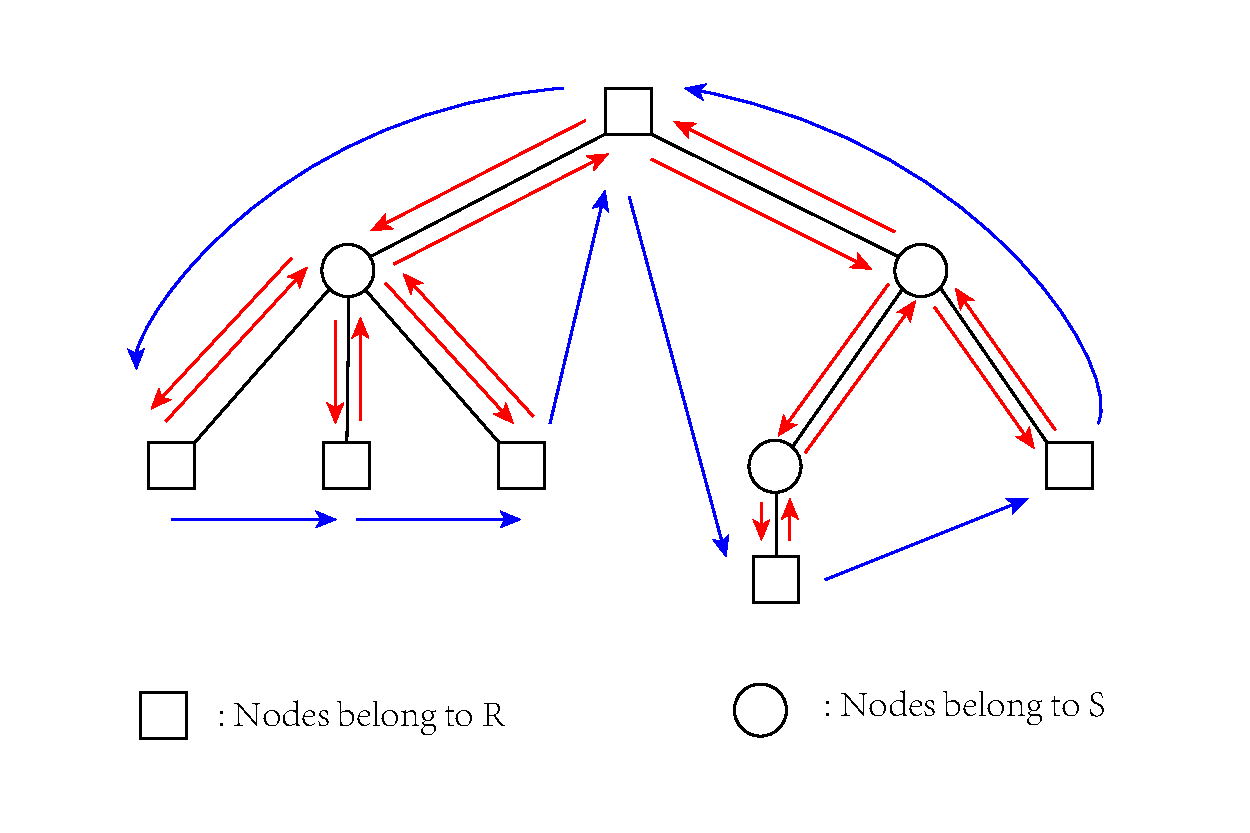
\includegraphics[width=0.8\textwidth]{pictures/01.pdf}
        \caption{\textbf{How to convert OPT Tree to MST on R}}\label{Graph1}
    \end{figure}
    \end{proof}

    \item
    \textbf{Minimum Weighted Vertex Cover:} Consider the weighted version of the Minimum Vertex Cover problem in which a non-negative weight $c_i$ is associated with each vertex $v_i$ and we look for a vertex cover having minimum total weight.\\

    \begin{enumerate}
        \item
        Given a weighted graph $G=(V, E)$ with a non-negative weight $c_i$ associated with each vertex $v_i$, please formulate the Minimum Weighted Vertex Cover problem as an integer linear program.\\ 
        \item
        Prove that the following algorithm finds a feasible solution of the Minimum Weighted Vertex Cover problem with value $m_{LP}(G)$ such that $m_{LP}(G)/m^*(G) \leq 2$.

        \begin{minipage}{0.8\textwidth}
        \centering
        \begin{algorithm}[H]
        \caption{Rounding Weighted Vertex Cover}
        \KwIn{Graph $G=(V, E)$ with non-negative vertex weights;}
        \KwOut{Vertex cover $V'$ of $G$;}
        \BlankLine
        Let $ILP_{VC}$ be the integer linear programming formulation of the problem\;
        Let $LP_{VC}$ be the problem obtained from $ILP_{VC}$ by LP-relaxation\;
        Let $x^*(G)$ be the optimal solution for $LP_{VC}$\;
        $V' \leftarrow \{v_i \ | \ x_i^*(G) \geq 0.5\}$\;
        \Return{$V'$};
        \end{algorithm}
        \end{minipage}

    \end{enumerate}

    \begin{solution}\item
    \renewcommand{\qedsymbol}{}
    \begin{itemize}
    \item [(a)] First and Foremost, we define a variable $x_{i}$ for each vertex $v_{i}$, which equals 1 ($x_{i}=1$) iff $v_{i}$ is chosen to be included in a vertex cover, otherwise $x_{i}=0$.\par Then, the minimum weighted vertex cover can be formulated as the following integer linear program: \\

    \qquad\textbf{minimize.}
    $$\sum_{v=1}^{|V|}c_{i}x_{i} $$
    \qquad\textbf{subject to.}
    $$x_{i}+x_{j} \geq 1, \forall e=(v_i,v_j)\in E$$
    $$x_{i}\in \{0,1\}, \forall v_i\in V $$\\

    For section (2), we we can relax the constraint $x_{i}\in \{0,1\}$ to $x_{i}\in [0,1]$. Futhermore, we can give up the redundant constraint $x_{i}\leq 1$ to get  simplified edition $x_{i}\geq 0, \forall v_i\in V $. LP approximation can be summed as follow:\\

    \qquad\textbf{minimize.}
    $$\sum_{v=1}^{|V|}c_{i}x_{i} $$
    \qquad\textbf{subject to.}
    $$x_{i}+x_{j} \geq 1, \forall e=(v_i,v_j)\in E$$
    $$x_{i}\geq 0, \forall v_i\in V$$\\
    \item [(b)] \textbf{Proof.}\par
    \begin{itemize}
    \item (Feasible Solution) For any edge $e = (v_i, v_j) \in E$, by feasibility of $x^*$, $x_{i}^*+x_{j}^* \geq 1$, which means either $x_{i}^*\geq 
    \frac{1}{2}$ or $x_{j}^*\geq \frac{1}{2}$. Therefore, at least one of $x_{i}$ and $x_{j} $ will be in vertex cover set $V'$.
    \item (Approximation Ratio) According to LP, we have
    $$m^*(G)=\sum_{v=1}^{|V|}c_{i}x_{i}^*\geq \frac{1}{2} \sum_{v_i\in V'}{c_{i}}=\frac{1}{2} m_{LP}(G) $$
    it obviously prove that
    $m_{LP}(G)/m^*(G) \leq 2$.
    \end{itemize}
    \end{itemize}
    \end{solution}

    \item
    Give the corresponding $(I,sol,m,goal)$ for \textbf{Metric $k$-center} and \textbf{Minimum Weighted Vertex Cover} respectively.

    \begin{solution}\item
    \renewcommand{\qedsymbol}{}
    \begin{itemize}
    \item 
    \textbf{Metric k-center}:\par
    (1) $I=\{(I_1, I_2,k)|\ k\geq 0, \cdots\}$;\par
    $I_1 = \{G = (V,E) |G\ is\ a\ graph\}$, $I_2 = \{C = (e_i,c_i) |\ e_i\in E, c_i\geq 0, c_i\in triangle\ inequality\}$;\par
    (2) $sol(G, k)=\{S \subseteq V|\ |S| = k\}$;\ \ \ (feasible solution set and poly-time decidable)\par
    (3) $m(G, C, S) = \max_v\{cost(v, S)\}$;\ \ \ (poly-time computable function)\par
    (4) goal = min.
    \item 
    \textbf{Minimum Weighted Vertex Cover}:\par
    (1) $I=\{(I_1, I_2)| \cdots\}$;\par $I_1 = \{G = (V,E) |\ G\ is\ a\ graph\}$, $I_2 = \{C = (v_i,c_i) |\ v_i\in V, c_i\geq 0 \}$;\par
    (2) $sol(G)=\{S\subseteq V\ |\ \forall(v_i,v_j)\in E[v_i \in S \vee v_j\in S]\}$;\ \ \ (feasible solution set and poly-time decidable)\par
    (3) $m(G, C, S) = \sum_{v_i\in S,\ (v_i,c_i)\ exist}(c_i) $;\ \ \ (poly-time computable function)\par
    (4) goal = min.
    \end{itemize}
    \end{solution}

\end{enumerate}

\vspace{20pt}



%========================================================================
\end{document}
